
\section{General counter}


\begin{figure}[H]
    \centering
    \begin{subfigure}[t]{0.2\textwidth}
        \centering
        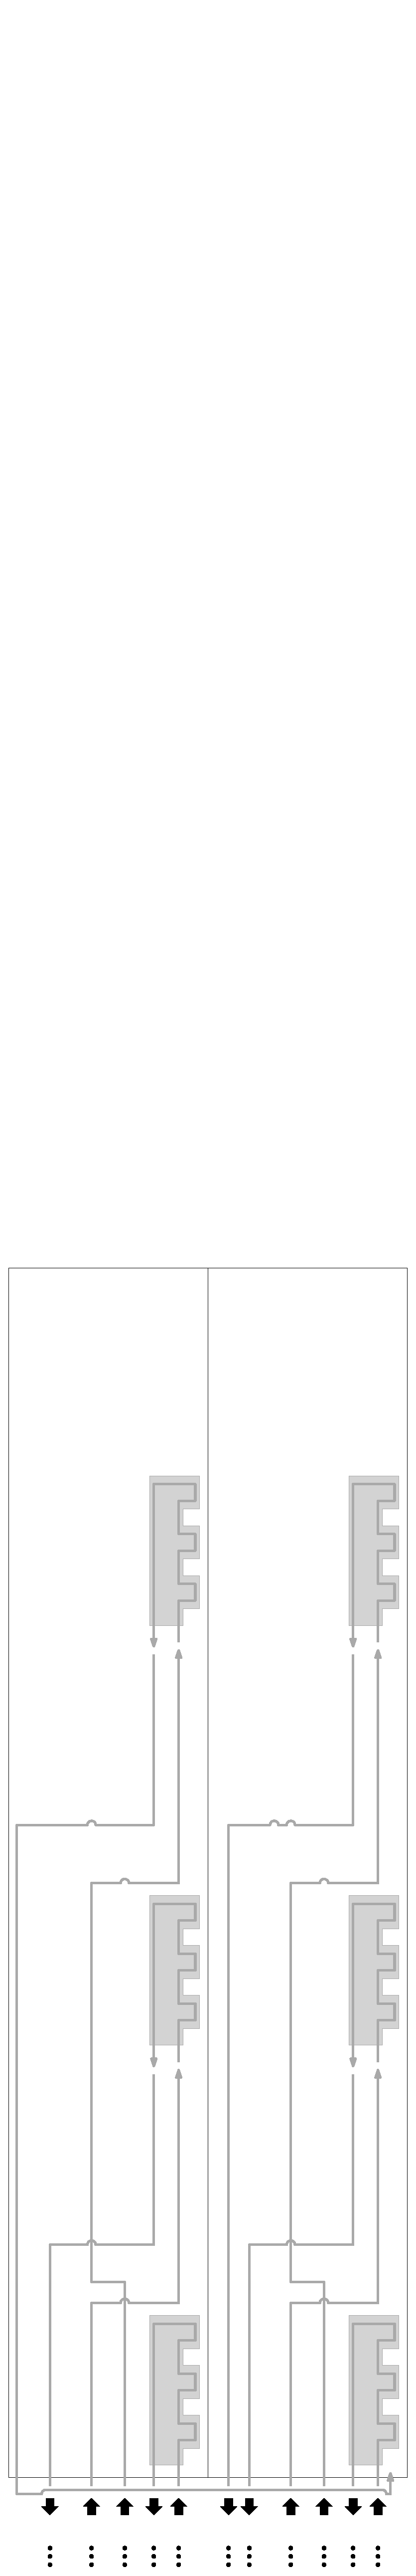
\includegraphics[width=0.6in]{counter_read_start_general_case3_middle_level}
        \caption{\label{fig:counter_read_start_general_case3_middle_level} A ``clean'' counter row, before any reading has started.}
    \end{subfigure}%
    ~
    \begin{subfigure}[t]{0.2\textwidth}
        \centering
        \includegraphics[width=0.6in]{counter_read_digit1_return_read_digit2_general_case3_middle_level}
        \caption{\label{fig:counter_read_digit1_return_read_digit2_general_case3_middle_level} Read digit 1 in the current row, write digit 1 in the next row.}
    \end{subfigure}%
    ~
    \begin{subfigure}[t]{0.2\textwidth}
        \centering
        \includegraphics[width=0.6in]{counter_read_digit2_return_read_digit3_general_case3_middle_level}
        \caption{\label{fig:counter_read_digit2_return_read_digit3_general_case3_middle_level} Read digit 2 in the current row, write digit 2 in the next row.}
    \end{subfigure}%
    ~
    \begin{subfigure}[t]{0.2\textwidth}
        \centering
        \includegraphics[width=0.6in]{counter_read_digit3_return_read_digit1_general_case3_middle_level}
        \caption{\label{fig:counter_read_digit3_return_read_digit1_general_case3_middle_level} Read digit 3 in the current row, write digit 3 in the next row.}
    \end{subfigure}%

    \caption{\label{fig:counter_read_digit_return_read_digit_general_case3}
    This illustrates how a counter reads and writes a digit region, in a general sense.
    The counter starts in the rightmost digit region by reading the bottommost digit within
    that region. After reading digit 1 in the current row, the corresponding digit region in
    the next row be started in the next row. The counter writes the first digit in the next
    row, and then returns to the second digit in the current digit region.
    Once all the digits in the current digit region are read and written into the next row,
    the counter can then do one of the following: continue reading digits by moving on to the
    next digit region, cross back all the way to the right of the rectangle and start reading
    the next row, or halt.}
\end{figure}


\subsection{ Digit region explanation (in progress) }

Each logical row of the counter is made up of $\ceil*{\frac{d}{3}}$ ``digit regions". A digit region
is a group of 1-3 digits, stacked on top of each other vertically. Within a digit region, the digits are
sorted in order of significance, thus the most signifcant digit will be the topmost digit in that region,
the middle digit will have the second highest significance and finally the bottommost digit is the least
signifcant.

The leftmost digit region is most signifcant and the rightmost is the least signifcant.
The counter reads the least signifcant digit (1) in digit region 1, and continues in the current row
until it detects the final digit, in the MSR...

\begin{figure}[H]
    \centering
    \begin{subfigure}[t]{0.48\textwidth}
        \centering
        \includegraphics[width=2in]{digits_normal_counter}
        \caption{\label{fig:digits_normal_counter} Digits in a typical counter}
    \end{subfigure}%
    ~
    \begin{subfigure}[t]{0.48\textwidth}
        \centering
        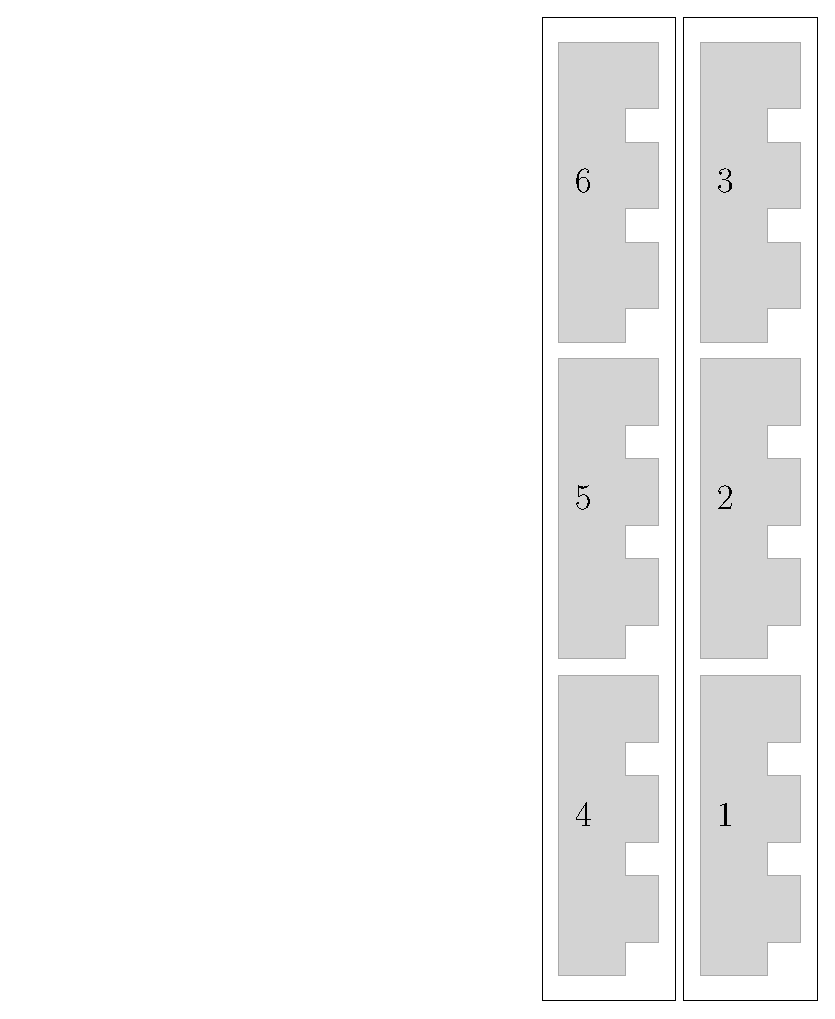
\includegraphics[width=2in]{digits_digit_region_counter}
        \caption{\label{fig:digits_digit_region_counter} Digits in two digit regions, stacked vertically, minimizing the width. }
    \end{subfigure}%
    ~
\end{figure}

Contrary to a typical counter, each counter row has an approximate height of 3 digits.
The digits are stacked up to 3 before increasing the width..